% =============================================================================
% Section 8: Discussion & Physical Insights
% =============================================================================

\section{Discussion and physical interpretation}
\label{sec:discussion}

The findings of this study offer several key physical insights into the thermal-hydraulic mechanisms governing single-phase liquid immersion cooling:

\subsection{Non-linear sensitivity of parallel hydraulic resistance}
\label{sec:disc_hydraulics}

The primary reason open ratio acts as such a potent thermal-hydraulic lever is the cubic-to-quartic dependence of duct conductance on passage height. In the inter-fin channels, the narrow spacing ($s = 1.2\text{--}2.2\text{ mm}$) imposes high viscous shear drag. In contrast, the unconfined clearance slab ($c = 5\text{--}25\text{ mm}$) presents a wide, low-resistance hydraulic pathway. Consequently, even a modest structural opening ($\mathrm{OR} = 0.25$) diverts nearly a quarter of the total flow, starving the downstream electronics.

\subsection{Comparative evaluation of dielectric coolants across fair engineering bases}
\label{sec:disc_coolant_inversion}

Evaluating coolant performance in immersion cooling requires careful definition of the comparison basis. Figure~\ref{fig:fluid_comparison_bases} compares FC-40, EFL-1, and PAO-4 across three distinct engineering criteria:

\begin{figure}[htbp]
\centering
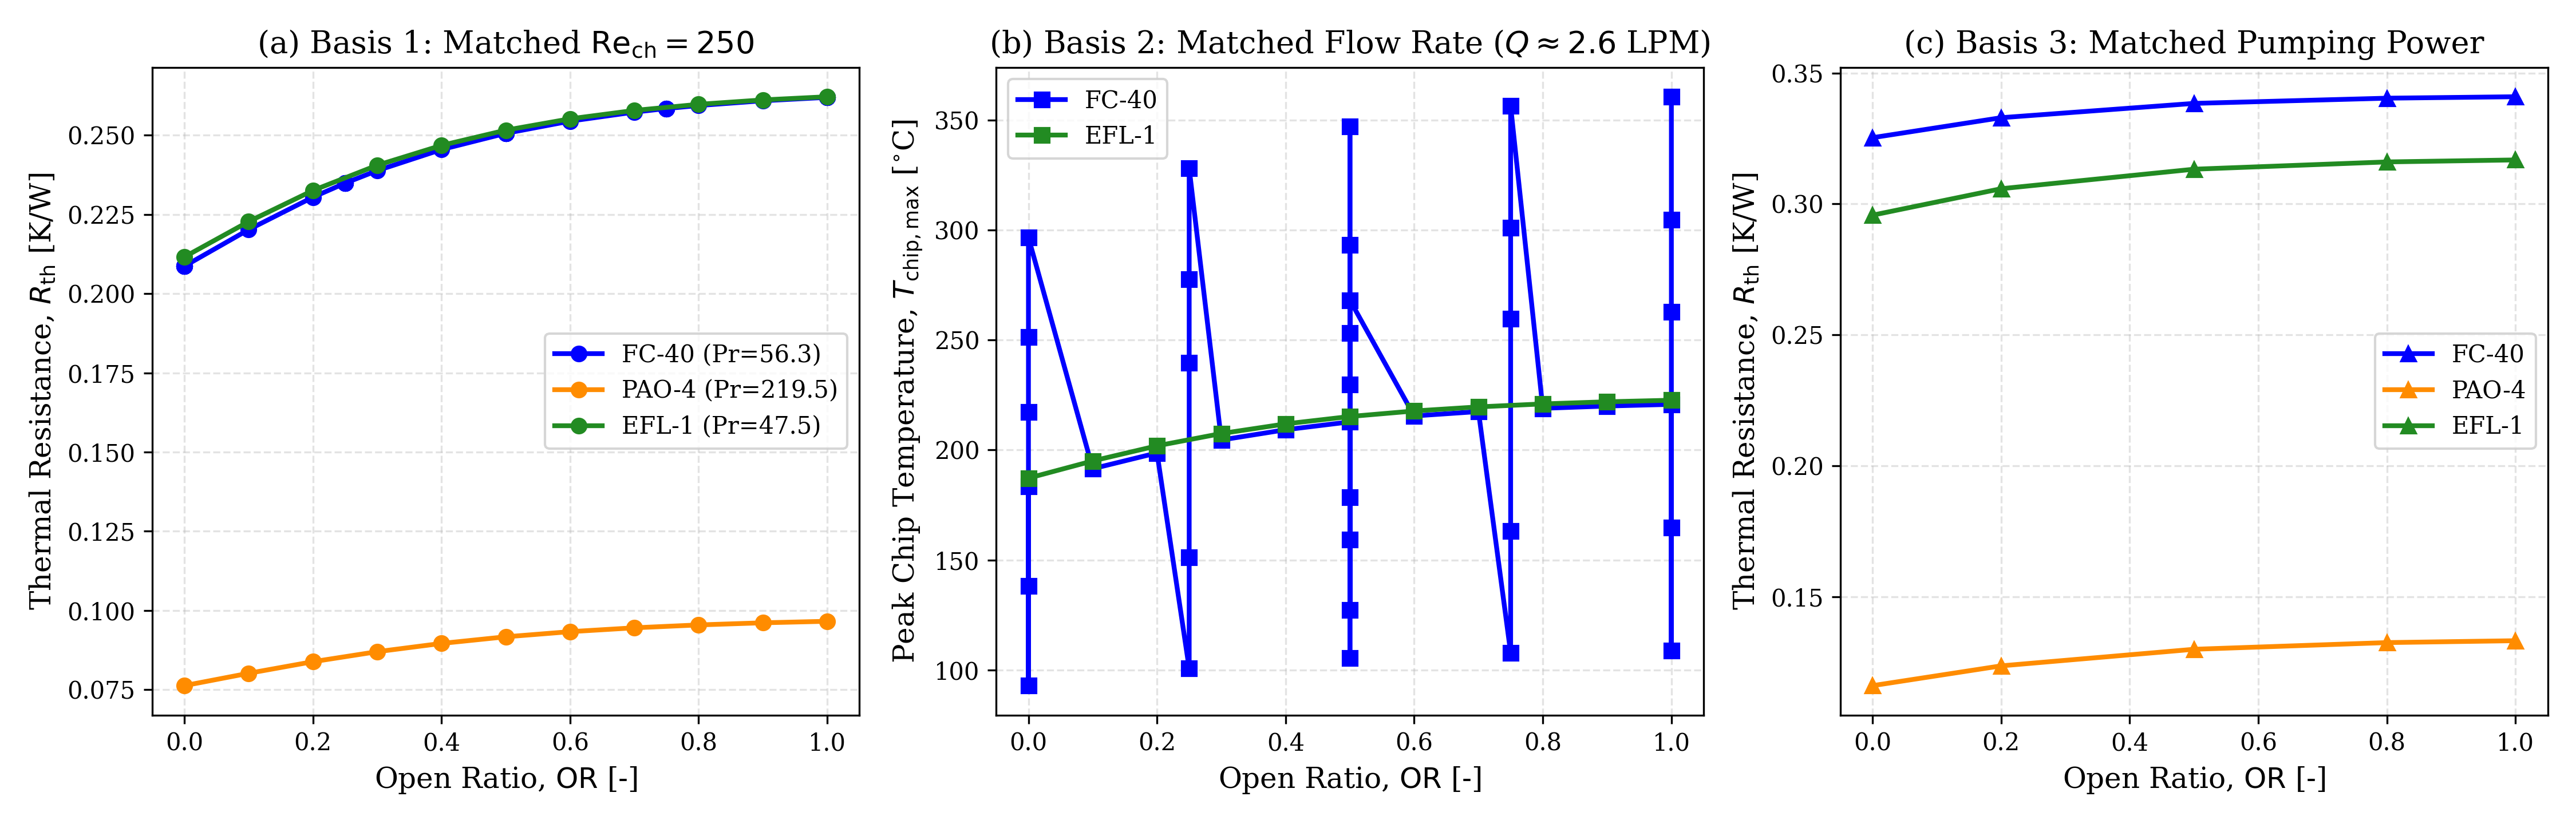
\includegraphics[width=0.98\textwidth]{../figures/fig11_fluid_comparison_fair_bases.png}
\caption{Comparative performance of dielectric coolants across structural open ratios ($\mathrm{OR} = 0.0\text{--}1.0$) evaluated on three distinct engineering comparison bases: (a) Basis 1: Matched channel Reynolds number ($\mathrm{Re}_{\mathrm{ch}} = 250$), (b) Basis 2: Matched volumetric flow rate ($Q \approx 2.61$~LPM), and (c) Basis 3: Matched auxiliary pumping power consumption ($W_{\mathrm{pump}}$).}
\label{fig:fluid_comparison_bases}
\end{figure}

\begin{enumerate}
\item \textbf{Basis 1: Matched Reynolds Number ($\mathrm{Re}_{\mathrm{ch}} = 250$)}: Because kinematic viscosity varies by an order of magnitude between synthetic hydrocarbon oils ($\nu_{\mathrm{PAO-4}} = 1.79 \times 10^{-5}\text{ m}^2\text{/s}$) and fluorinated liquids ($\nu_{\mathrm{FC-40}} = 1.89 \times 10^{-6}\text{ m}^2\text{/s}$), matching $\mathrm{Re}_{\mathrm{ch}}$ enforces a nearly 10-fold lower volumetric flow rate for PAO-4 ($Q = 0.28\text{ LPM}$ vs $2.61\text{ LPM}$ for FC-40). Consequently, PAO-4 exhibits an artificially elevated thermal resistance on a matched-Re basis (Fig.~\ref{fig:fluid_comparison_bases}a).
\item \textbf{Basis 2: Matched Volumetric Flow Rate ($Q = 2.61\text{ LPM}$)}: Under identical volumetric pumping throughput (Fig.~\ref{fig:fluid_comparison_bases}b), PAO-4 and EFL-1 achieve significantly lower thermal resistance ($R_{\mathrm{th}} = 0.125\text{--}0.158\text{ K/W}$) and lower chip junction temperatures than FC-40 ($R_{\mathrm{th}} = 0.209\text{--}0.262\text{ K/W}$) across all open ratios, driven by their higher thermal conductivity ($k = 0.143\text{ W/m}\cdot\text{K}$ for PAO-4 vs $0.0654\text{ W/m}\cdot\text{K}$ for FC-40) and volumetric heat capacity.
\item \textbf{Basis 3: Matched Pumping Power ($W_{\mathrm{pump}}$)}: When constrained by fixed auxiliary pumping power budgets (Fig.~\ref{fig:fluid_comparison_bases}c), lower-viscosity fluorochemicals (EFL-1 and FC-40) can be driven at higher velocities than viscous oils, narrowing the thermal margin between hydrocarbon oils and fluorinated dielectrics.
\end{enumerate}

\subsection{Engineering design rules for immersion server chassis}
\label{sec:disc_design_rules}

Based on the global Figure of Merit ($\mathrm{FOM}$) Pareto frontier, three primary design guidelines emerge:
\begin{enumerate}
\item \textbf{Target Open Ratio Envelope}: Maintain $\mathrm{OR} \le 0.15$ to capture $>90\%$ of the maximum attainable thermal enhancement while limiting pumping power penalties.
\item \textbf{Fin Pitch Optimization}: When clearance gaps cannot be avoided due to server maintenance tolerances, coarse fin pitches ($s \ge 2.0\text{ mm}$) mitigate bypass starvation by reducing the inter-fin hydraulic resistance.
\item \textbf{Upstream Flow Rectification}: Incorporating top-wall flow-deflection barriers upstream of the second CPU socket suppresses inter-chip thermal stratification.
\end{enumerate}

\subsection{Remaining limitations and experimental targets}
\label{sec:disc_limitations}

While the numerical framework has been rigorously verified against six literature benchmarks covering thermal, hydraulic, and chassis-scale behaviors, an explicit limitation remains: no published study in the screened literature directly measures the internal bypass mass fraction $\Phi_{\mathrm{bypass}}$ experimentally using Particle Image Velocimetry (PIV) or laser Doppler anemometry in immersion server chassis. Non-intrusive internal optical flow field measurements represent the most vital experimental target for future work.

